\documentclass[11pt]{article}

\usepackage[T1]{fontenc}
\usepackage{lmodern}
\usepackage[margin=0.82in]{geometry}
\usepackage{microtype}
\usepackage{xspace}
\usepackage{amsmath,amssymb,mathtools}
\usepackage{booktabs,tabularx,array,multirow}
\usepackage{enumitem}
\usepackage{xcolor}
\usepackage{graphicx}
\usepackage{tikz}
\usetikzlibrary{arrows.meta,positioning,fit,shapes.geometric}
\usepackage[style=authoryear,natbib=true,backend=biber,maxcitenames=2,maxbibnames=99]{biblatex}
\addbibresource{references.bib}
\usepackage[colorlinks=true,allcolors=blue!55!black]{hyperref}
\usepackage[nameinlink,noabbrev]{cleveref}
\usepackage{fancyhdr}
\usepackage{titlesec}
\usepackage{caption}

\definecolor{srblue}{HTML}{1F4E79}
\definecolor{srteal}{HTML}{0F766E}
\definecolor{srred}{HTML}{A63D40}
\definecolor{srgray}{HTML}{5B6573}
\definecolor{srlight}{HTML}{EEF4F8}

\hypersetup{
  pdftitle={SkillRewind: Recovering Hidden Influence Lineage for Verified Revocation in Self-Evolving LLM Agents},
  pdfauthor={Faisal Ali Said Al-Anqoudi},
  pdfsubject={Research Proposal},
  pdfkeywords={LLM agents, agent skills, provenance, causal replay, revocation, unlearning, security}
}

\pagestyle{fancy}
\fancyhf{}
\lhead{SkillRewind Research Proposal}
\rhead{Version 0.1 -- 9 August 2026}
\cfoot{\thepage}
\setlength{\headheight}{14pt}

\titleformat{\section}{\large\bfseries\color{srblue}}{\thesection}{0.55em}{}
\titleformat{\subsection}{\normalsize\bfseries\color{srteal}}{\thesubsection}{0.5em}{}
\setlist{nosep,leftmargin=1.35em}
\captionsetup{font=small,labelfont=bf}
\renewcommand{\arraystretch}{1.14}

\newcommand{\system}{\textsc{SkillRewind}\xspace}
\newcommand{\bench}{\textsc{RewindBench}\xspace}
\newcommand{\obs}{G_{\mathrm{obs}}}
\newcommand{\trueg}{G_{\star}}
\newcommand{\closure}{\mathcal{C}}
\newcommand{\artifacts}{\mathcal{V}}
\newcommand{\edges}{\mathcal{E}}

\begin{document}

\begin{center}
{\LARGE\bfseries\color{srblue} SkillRewind: Recovering Hidden Influence Lineage\\[2pt]
for Verified Revocation in Self-Evolving LLM Agents}\par
\vspace{0.55em}
{\large Research Proposal -- Version 0.1}\par
\vspace{0.75em}
{\bfseries Faisal Ali Said Al-Anqoudi}\par
Co-Founder \& CEO, Nuqta Technologies\par
Muscat, Oman\par
\vspace{0.55em}
9 August 2026
\end{center}

\vspace{0.4em}
\noindent\colorbox{srlight}{\parbox{0.97\linewidth}{\small\textbf{Evidence status.}
This document is a research proposal, not a results paper. It reports no fabricated experimental findings. Numerical results attributed to prior work are cited; all SkillRewind performance numbers are explicitly stated as hypotheses, evaluation targets, or go/no-go criteria.}}

\begin{abstract}
Self-evolving large-language-model agents increasingly distill trajectories, memories, tool interactions, and documents into persistent skills. Revoking a poisoned or obsolete source is therefore not a local deletion problem: its influence may survive in semantically rewritten descendants, multi-file skill packages, persistent memories, or generated code. Existing cascade-repair methods provide strong containment when the complete influence graph is known, but this assumption is fragile in deployed agents, where attribution edges may be missing because of incomplete instrumentation, cross-model distillation, lossy summarization, or legacy skill imports. We propose \system, a framework for revoking persistent agent behavior under incomplete provenance. \system combines recorded derivation edges, multi-trace candidate recovery over expression, implementation, operational structure, and behavior, and budgeted counterfactual re-derivation to confirm uncertain influence relationships. Confirmed descendants are quarantined or rebuilt from clean support, then subjected to paired utility and safety validation. The system emits a bounded revocation attestation that distinguishes recorded facts, inferred relationships, replay-confirmed effects, repaired artifacts, and unresolved uncertainty. We further propose \bench, a benchmark with planted lineage ground truth, controlled provenance loss, semantic laundering, code mutation, multi-hop contamination, cross-model distillation, and compositional influence. The central research question is whether active lineage recovery can substantially reduce residual poisoned behavior while preserving more clean utility and using fewer model calls than exhaustive replay or conservative cascade deletion.
\end{abstract}

\section{Motivation and Research Gap}

Agent Skills are portable directories centered on a \texttt{SKILL.md} file and may include executable scripts, references, assets, and arbitrary metadata \citep{agentskills2026}. This representation is becoming a practical substrate for procedural memory: recent systems automatically discover, distill, refine, and share skills from agent experience \citep{skillrl2026,trace2skill2026,skillclaw2026,coevoskills2026}. The resulting capability is valuable, but it creates a new lifecycle problem. A transient observation can be promoted into a durable instruction artifact and can later influence tasks even after the original observation is removed.

Recent attacks demonstrate that this is not merely hypothetical. SkillJack shows that poisoned trajectories can be transformed into durable skills whose malicious intent becomes less detectable and whose behavior often persists after deletion of the source records \citep{skilljack2026}. PoisonedEvolution independently targets evidence promotion in SkillClaw and Trace2Skill, showing that bounded attacker support can be attributed as reusable expertise and embedded into evolved skill artifacts \citep{poisonedevolution2026}. At ecosystem scale, public skills also contain substantial instruction, executable, and supply-chain risk \citep{skillswild2026}.

The closest repair formulation is MemoRepair, which withdraws the descendant cascade of an invalidated artifact, rebuilds successors from retained support, and republishes only validated predecessor-closed artifacts \citep{memorepair2026}. Its guarantee, however, depends on complete influence provenance. The paper reports that dropping only 1\% of influence edges produces 17.7\% leakage, making missing lineage a first-order failure mode rather than a minor implementation issue. Related systems provide important but different primitives: MemLineage records cryptographic memory lineage and gates sensitive actions \citep{memlineage2026}; NeuroTaint reconstructs semantic, causal, and cross-session source-to-sink propagation in execution traces \citep{neurotaint2026}; SkillTrace audits transformed reuse through expression, implementation, and operational traces \citep{skilltrace2026}; SkillWiki supplies lifecycle and provenance infrastructure \citep{skillwiki2026}; and Agentic Unlearning jointly addresses parametric and memory pathways \citep{agenticunlearning2026}.

\paragraph{Working novelty hypothesis.}
To the best of the literature review completed for this proposal, no published system treats the following four elements as one revocation contract: (i) persistent self-evolved skill artifacts, (ii) missing influence edges, (iii) active interventional recovery of uncertain lineage, and (iv) selective cascade rebuilding followed by a bounded, evidence-typed attestation. This claim will be re-audited immediately before submission and narrowed if concurrent work overlaps.

\begin{table}[t]
\centering
\small
\caption{Positioning against the closest published systems. ``Recovered'' denotes missing or unrecorded lineage; ``Replay'' denotes an active intervention rather than passive trace comparison.}
\label{tab:landscape}
\begin{tabularx}{\linewidth}{@{}l>{\raggedright\arraybackslash}Xccccc@{}}
\toprule
System & Primary object & Recorded & Recovered & Replay & Rebuild & Attest. \\
\midrule
MemoRepair & Derived memory and skills & Yes & No & No & Yes & No \\
MemLineage & Persistent memory entries & Yes & No & No & No & Log \\
NeuroTaint & Source-to-sink execution influence & Partial & Partial & Analysis & No & Path \\
SkillTrace & Reused skill packages & Post hoc & Yes & No & No & Report \\
Agentic Unlearning & Parameters and memory & Closure & No & No & Logical & No \\
SkillWiki & Skill lifecycle ecosystem & Yes & No & No & Workflow & Records \\
\textbf{SkillRewind} & Persistent skills, memories, and derived artifacts & Yes & \textbf{Yes} & \textbf{Yes} & \textbf{Yes} & \textbf{Yes} \\
\bottomrule
\end{tabularx}
\end{table}

\section{Problem Formulation}

Let $\artifacts$ be immutable versions of persistent artifacts: trajectories, memories, summaries, skill directories, prompt patches, code, templates, and validation records. Let the latent influence graph be
\[
\trueg=(\artifacts,\edges_{\star}),
\]
where $(u,v)\in\edges_{\star}$ means that artifact $u$ had behaviorally relevant causal influence on the derivation of $v$. Instrumentation exposes only
\[
\obs=(\artifacts,\edges_{\mathrm{obs}}), \qquad \edges_{\mathrm{obs}}\subseteq\edges_{\star}.
\]
For revoked roots $F\subseteq\artifacts$, the true affected closure is
\[
\closure_{\star}(F)=\{v\in\artifacts:\exists f\in F\text{ such that }f\leadsto v\text{ in }\trueg\}.
\]
The system must estimate $\widehat{\closure}(F)$, quarantine or repair affected artifacts, and preserve unaffected utility while operating under a finite replay budget $B$.

A simplified research objective is
\[
\min_{\widehat{\closure},\,Q,\,R}
\alpha\,|\closure_{\star}\setminus\widehat{\closure}|+
\beta\,|\widehat{\closure}\setminus\closure_{\star}|+
\lambda\,\mathrm{Cost}_{\mathrm{replay}}(Q)+
\mu\,\mathrm{Cost}_{\mathrm{repair}}(R),
\]
where the first term penalizes missed contaminated descendants, the second penalizes false quarantine, $Q$ is the set of counterfactual tests, and $R$ is the selected repair plan. In controlled experiments, $\closure_{\star}$ is known. In real deployments it is not; therefore, the production output must expose evidence and uncertainty rather than claim perfect unlearning.

\paragraph{Replayability boundary.}
The main causal claim applies when the derivation episode is replayable: the system retains a task snapshot, evolver configuration, candidate context pool, model identifier, and environment digest, even if explicit influence edges are missing. Legacy artifacts without such snapshots are handled in forensic mode; they may receive static evidence scores but cannot receive replay-confirmed causal status.

\section{Research Questions and Hypotheses}

\begin{description}[leftmargin=1.4em,labelindent=0pt,style=nextline]
\item[RQ1: Hidden-descendant recovery.] Can multi-trace evidence recover descendants whose explicit provenance edges are missing under semantic, implementation, and operational transformations?
\item[RQ2: Causal confirmation under budget.] Can active counterfactual replay approach exhaustive-replay accuracy while using substantially fewer re-derivations?
\item[RQ3: Revocation effectiveness.] Does selective quarantine and clean-room rebuilding reduce residual harmful behavior more than source deletion, recorded-closure traversal, or static similarity alone?
\item[RQ4: Utility and calibration.] Can the system preserve clean task utility and produce confidence estimates that remain calibrated across models, evolution pipelines, and provenance-loss regimes?
\end{description}

The directional hypotheses are: (H1) fusing expression, implementation, operational, behavioral, and graph evidence will outperform text embeddings alone; (H2) information-gain-based replay selection will dominate random or uncertainty-only selection at equal budget; (H3) replay-confirmed cascade repair will reduce residual canary activation while preserving more clean utility than conservative deletion; and (H4) evidence-typed attestations will have materially higher coverage than recorded provenance alone without presenting inferred edges as deterministic facts.

\section{Proposed System}

\begin{figure}[t]
\centering
\resizebox{0.98\linewidth}{!}{%
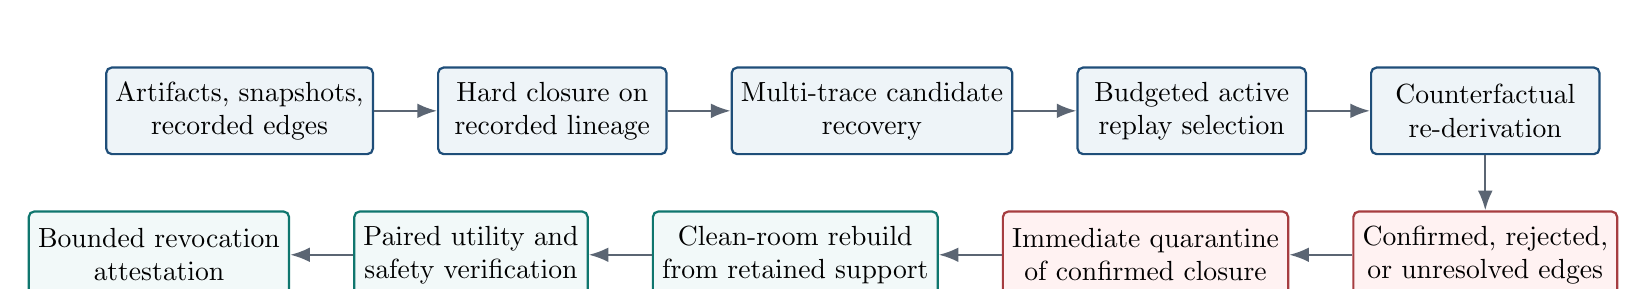
\begin{tikzpicture}[
  node distance=7mm and 8mm,
  box/.style={draw=srblue, rounded corners=2pt, thick, align=center, minimum height=11mm, minimum width=29mm, fill=srlight},
  risk/.style={draw=srred, rounded corners=2pt, thick, align=center, minimum height=11mm, minimum width=29mm, fill=red!5},
  good/.style={draw=srteal, rounded corners=2pt, thick, align=center, minimum height=11mm, minimum width=29mm, fill=teal!5},
  arrow/.style={-{Latex[length=2.5mm]}, thick, draw=srgray}
]
\node[box] (capture) {Artifacts, snapshots,\\recorded edges};
\node[box, right=of capture] (hard) {Hard closure on\\recorded lineage};
\node[box, right=of hard] (trace) {Multi-trace candidate\\recovery};
\node[box, right=of trace] (select) {Budgeted active\\replay selection};
\node[box, right=of select] (replay) {Counterfactual\\re-derivation};
\node[risk, below=of replay] (classify) {Confirmed, rejected,\\or unresolved edges};
\node[risk, left=of classify] (quarantine) {Immediate quarantine\\of confirmed closure};
\node[good, left=of quarantine] (rebuild) {Clean-room rebuild\\from retained support};
\node[good, left=of rebuild] (verify) {Paired utility and\\safety verification};
\node[good, left=of verify] (attest) {Bounded revocation\\attestation};
\draw[arrow] (capture) -- (hard);
\draw[arrow] (hard) -- (trace);
\draw[arrow] (trace) -- (select);
\draw[arrow] (select) -- (replay);
\draw[arrow] (replay) -- (classify);
\draw[arrow] (classify) -- (quarantine);
\draw[arrow] (quarantine) -- (rebuild);
\draw[arrow] (rebuild) -- (verify);
\draw[arrow] (verify) -- (attest);
\end{tikzpicture}}
\caption{Proposed SkillRewind pipeline. Recorded lineage yields a deterministic hard closure. Multi-trace evidence generates candidates for missing edges; active counterfactual re-derivation confirms only the most informative candidates under budget.}
\label{fig:architecture}
\end{figure}

\subsection{Immutable Capture and Hard Closure}
Every persisted artifact receives a content digest and a derivation manifest. The manifest records the recipe, model and decoding configuration, environment digest, candidate context set, retrieved memories, active skills, input trajectories, tool outputs, and validation suite. Exact ``used-as-input'' edges form the hard graph. On revocation, the system immediately withdraws the recorded descendant closure before any probabilistic analysis, following the barrier-first principle of MemoRepair \citep{memorepair2026}.

\subsection{Multi-Trace Candidate Recovery}
For every earlier artifact $u$ and later artifact $v$ within a bounded temporal and task neighborhood, the candidate generator computes complementary evidence:
\begin{itemize}
\item \textbf{Expression trace:} normalized prose, activation cues, examples, and instruction fragments using lexical fingerprints and semantic embeddings.
\item \textbf{Implementation trace:} normalized abstract syntax trees, API-call signatures, command structures, data-flow summaries, and configuration schemas.
\item \textbf{Operational trace:} a typed graph of activation conditions, procedural steps, tools, resources, and artifact flows, extending the operational-birthmark insight of SkillTrace \citep{skilltrace2026}.
\item \textbf{Behavioral trace:} a vector of deterministic probe outcomes, tool-call patterns, side effects in a sandbox, and policy-relevant canary activations.
\item \textbf{Graph and temporal priors:} shared tasks, overlapping candidate context pools, common evolver recipes, version adjacency, and ancestry through already confirmed edges.
\end{itemize}
A calibrated model produces $p_{uv}=P((u,v)\in\edges_{\star}\mid x_{uv})$. Same-function independent skills are mandatory strict negatives so that common functionality is not mistaken for inheritance.

\subsection{Budgeted Counterfactual Re-Derivation}
Static similarity is insufficient for a causal revocation decision. For replayable derivations, \system restores the pre-derivation snapshot and runs paired interventions with the candidate ancestor available and withheld or replaced by a clean control. Let $Y^{+u}$ and $Y^{-u}$ denote distributions over the derived artifact and its behavior. The estimated effect is
\[
\widehat{\Delta}_{u\rightarrow v}=\mathbb{E}\left[d(Y^{+u},Y^{-u})\right],
\]
where $d$ combines deterministic verifier changes, normalized AST or graph differences, behavioral probe divergence, and target canary activation. Repeated seeds produce confidence intervals when the evolver is stochastic. The method adopts the intervention-first principle of Causal Agent Replay \citep{causalreplay2026}, but applies it to artifact derivation rather than step-level failure attribution.

Because exhaustive pairwise replay is expensive, candidates are selected by expected information gain divided by estimated cost. The selector prioritizes bridge edges whose confirmation would change the largest uncertain descendant closure. Pairwise or Monte-Carlo Shapley tests are reserved for top-ranked compositional cases where no single ancestor has a sufficient marginal effect.

\subsection{Quarantine, Clean-Room Rebuild, and Verification}
Confirmed descendants are made non-servable. Rebuilding replays the original recipe using only retained, non-revoked support and repaired predecessors. A successor is republished only if it passes: (i) task-specific deterministic verifiers, (ii) paired no-skill or clean-skill utility tests, (iii) safety probes targeted to the revoked behavior, and (iv) predecessor-closure checks. Artifacts that cannot be replayed or validated remain quarantined rather than being silently restored.

\subsection{Bounded Revocation Attestation}
The output is a machine-readable and human-readable attestation with four evidence classes:
\begin{enumerate}
\item \textbf{Recorded:} edges and descendants directly captured by instrumentation.
\item \textbf{Inferred:} candidate relationships supported by static multi-trace evidence.
\item \textbf{Replay-confirmed:} relationships with intervention effects and confidence intervals.
\item \textbf{Unresolved:} artifacts outside the replayability or validation boundary.
\end{enumerate}
The strongest permitted claim is therefore bounded: no active artifact remains in the recorded and replay-confirmed closure, and no target behavior was observed under the declared probe suite. This is not a claim of exact parameter erasure or universal semantic unlearning.

\section{RewindBench}

\bench will provide planted lineage ground truth and a real-system track.

\subsection{Benchmark Tracks}
\textbf{Core controlled track.} A generator creates derivation DAGs of depth 1--5 with known ancestors, benign utility, and inert security canaries. It produces both direct and transformed descendants while recording a complete oracle graph. The benchmark then removes edges according to controlled missingness policies.

\textbf{System track.} Adapters instrument two public self-evolution pipelines, initially SkillClaw and Trace2Skill \citep{skillclaw2026,trace2skill2026}. CoEvoSkills is an optional third system because it produces multi-file skill packages and uses an independent verifier \citep{coevoskills2026}. The evaluation will use pinned commits, container digests, and model snapshots.

\subsection{Scenario Families}
\begin{table}[t]
\centering
\small
\caption{Planned RewindBench scenario families. All harmful effects are inert canaries or mocked side effects executed in isolated sandboxes.}
\label{tab:scenarios}
\begin{tabularx}{\linewidth}{@{}lX@{}}
\toprule
Family & What survives transformation \\
\midrule
Direct inheritance & Instruction or code is copied with light edits. \\
Semantic laundering & The same unsafe rule is paraphrased without distinctive lexical overlap. \\
Implementation mutation & Code is rewritten, translated, or moved to a different API while preserving behavior. \\
Procedural inheritance & The operational sequence or trust assumption survives even when text and code change. \\
Multi-hop contamination & Influence passes through two to five generations of skills or memories. \\
Memory-to-skill promotion & A persistent memory or summary is distilled into a reusable skill. \\
Cross-model distillation & One model generates a skill that a different model later revises or consolidates. \\
Compositional influence & The target effect appears only when two otherwise benign ancestors are jointly present. \\
\bottomrule
\end{tabularx}
\end{table}

\subsection{Provenance-Loss Regimes}
The benchmark will evaluate edge dropout at 0, 1, 5, 10, 25, and 50\%. Missingness will be: (i) uniform random; (ii) type-selective, such as dropping memory-to-skill edges; (iii) bridge-targeted, removing high-betweenness edges; and (iv) attribution-selective, removing edges most likely to be omitted by an evolver that only records explicitly cited evidence. This distinguishes robustness to accidental logging gaps from adversarial or structurally biased incompleteness.

\section{Experimental Design}

\subsection{Baselines}
The planned baselines are:
\begin{enumerate}
\item \textbf{DeleteRoot:} delete only the revoked source.
\item \textbf{RecordedClosure:} traverse only observed influence edges; this isolates the complete-provenance assumption.
\item \textbf{Embedding:} semantic text similarity with calibrated thresholds.
\item \textbf{StaticMultiTrace:} expression, implementation, operational, and behavioral fusion without replay.
\item \textbf{ExhaustiveReplay:} replay every candidate pair within the oracle candidate window; an expensive upper-bound baseline.
\item \textbf{SkillRewind-Active:} the proposed active selector plus counterfactual re-derivation, quarantine, rebuilding, and verification.
\end{enumerate}
Where public implementations are compatible, the study will also compare or interoperate with MemoRepair, SkillTrace, and NeuroTaint rather than presenting reimplementations as exact replicas.

\subsection{Primary Metrics}
\begin{itemize}
\item Hidden-descendant recall, precision, F1, and path-level recall.
\item Residual canary attack success rate after revocation and repair.
\item False quarantine rate and retained clean utility.
\item Repair success rate and fraction of successors safely republished.
\item Replay calls, tokens, wall-clock time, and cost-normalized recall.
\item Calibration using Brier score, expected calibration error, and reliability diagrams.
\item Attestation coverage: recorded, inferred, replay-confirmed, and unresolved fractions.
\end{itemize}

\subsection{Pre-Registered Success Criteria}
These are targets, not claims. At 10\% random provenance loss, the primary go/no-go criteria are: (i) hidden-descendant recall at least 0.85 with false quarantine at most 0.10; (ii) residual canary activation at most 5\% after repair while retaining at least 90\% of clean utility relative to the pre-revocation system; (iii) at least 90\% of ExhaustiveReplay F1 using no more than 40\% of its replay calls; and (iv) expected calibration error no greater than 0.10. Failure to meet a criterion will be reported directly and used to narrow the claims.

\subsection{Statistical Protocol}
Conditions will be paired on the same tasks, seeds, derivation snapshots, and candidate graphs. Rates will receive Wilson or bootstrap 95\% confidence intervals. McNemar tests will compare paired detection outcomes; paired bootstrap tests will compare utility; and mixed-effects logistic regression will model system, model family, scenario, depth, and missingness level. Holm correction will control family-wise error across the pre-registered primary comparisons. All prompts, seeds, container digests, raw traces, and analysis scripts will be released when licenses permit.

\subsection{Ablations}
Ablations will remove each trace family, replace active selection with random and uncertainty-only policies, disable graph priors, disable interaction testing, vary replay repetitions, and replace clean-room rebuilding with deletion-only containment. A separate replay-fidelity study will measure whether model or environment drift changes the inferred edge labels.

\section{Threat Model, Limitations, and Ethics}

The adversary may inject or influence bounded trajectories, documents, memories, or tool outputs that enter a skill-evolution pipeline, but cannot modify the SkillRewind log, experiment harness, or ground-truth labels. The defender may revoke an artifact after deployment and has access to captured snapshots within the declared replayability boundary.

The proposal has important limitations. Counterfactual claims depend on faithful replay; closed hosted models, undocumented model updates, nondeterministic tools, or missing environment state can invalidate that assumption. Multi-trace similarity can confuse independent solutions with inheritance. Interaction effects may exceed the replay budget. The method governs externalized skills and memory artifacts; it does not guarantee removal from foundation-model weights. Passing a finite verifier suite does not prove correctness in all future contexts.

All benchmark payloads will be inert: for example, emitting a canary token, selecting a mocked unsafe flag, or writing to a sandbox-only path. No real credentials, external accounts, destructive commands, or live exfiltration targets will be used. Newly discovered vulnerabilities in public evolution systems will follow coordinated disclosure before release of exploit details.

\section{Expected Contributions and Work Plan}

The intended contributions are:
\begin{enumerate}
\item a formal problem definition for skill revocation under incomplete influence provenance;
\item a hybrid recovery method combining multi-trace candidate generation with budgeted causal re-derivation;
\item a barrier-first quarantine and clean-room rebuild contract with evidence-typed attestations;
\item \bench, including controlled ground truth, realistic transformations, and provenance-loss regimes; and
\item an open-source reference implementation compatible with the Agent Skills format.
\end{enumerate}

\begin{table}[h]
\centering
\small
\caption{Initial 20-week execution plan. Milestones are ordered by dependency; experimental claims begin only after the benchmark and baselines are frozen.}
\label{tab:timeline}
\begin{tabularx}{\linewidth}{@{}lX@{}}
\toprule
Weeks & Deliverable \\
\midrule
1--2 & RFC, threat model, literature audit, artifact and attestation schemas. \\
3--5 & Content-addressed store, derivation capture, replayable snapshots, RecordedClosure baseline. \\
6--8 & RewindBench-Core generator, provenance-loss operators, deterministic canary verifiers. \\
9--11 & Multi-trace extraction, calibrated candidate generation, strict-negative mining. \\
12--14 & Counterfactual re-derivation, active selector, interaction tests, replay-cost accounting. \\
15--16 & Quarantine, clean-room rebuild, validation, and attestation implementation. \\
17--18 & System adapters, frozen experiment matrix, ablations, statistical analysis. \\
19--20 & Paper, artifact documentation, reproducibility audit, responsible disclosure, public release. \\
\bottomrule
\end{tabularx}
\end{table}

\section{Reproducibility Contract}

The repository will pin model and harness identifiers, preserve raw and normalized artifacts, separate benchmark-generation code from scoring code, and publish a manifest of every reported number. Deterministic components will be byte-checked in continuous integration. Hosted-model runs will be archived as signed logs and clearly separated from locally reproducible runs. The final paper will include a limitations checklist and an explicit mapping from each claim to the exact experiment, metric, and artifact that supports it.

\begingroup
\setlength{\emergencystretch}{3em}
\printbibliography[title={References}]
\endgroup

\end{document}
